\documentclass[aps,prb,onecolumn,notitlepage,showpacs,floatfix,superscriptaddress]{revtex4-1}
\usepackage{dcolumn}
\usepackage{tabularx}
\usepackage{bm}
\usepackage{soul}
\usepackage{amsmath,amssymb,graphicx}
\usepackage[colorlinks=true,citecolor=blue,urlcolor=blue,linkcolor=blue]{hyperref}
\usepackage{environ}

\NewEnviron{eqnsplit}{%
\begin{equation}
\begin{split}
  \BODY
\end{split}
\end{equation}
}

\newcommand{\mrm}[1]{\mathrm{#1}}
\newcommand{\ang}{\mathrm{\AA}}

\bibliographystyle{apsrev4-1}

%%%%%%%%%%%%%%%%%%%%%%%%%%%%%%%%%%%%%%%%%%%%%%%%
\begin{document}

\title{Pauli Paramagnetism}

\author{Avinash Rustagi}
\email{arustag@ncsu.edu}
\affiliation{Department of Physics, North Carolina State University, Raleigh, NC 27695}
%
\date{\today}
%%%%%%%%%%%%%%%%%%%%%%%%%%%%%%%%%%%%%%%%%%%%%%%%

\maketitle
%
In a non-magnetic system, we have equal number of spin up and spin down electrons ($n_{\uparrow}=n_{\downarrow}=n$). In presence of magnetic field, the Zeeman energy term shifts the bands which means that there is an imbalance of up and down spins creating a magnetization.\\

Let us consider a simple model with on-site repulsion (i.e. an energy cost $U$ when two electrons occupy the same site). As per the Pauli exclusion principle, it is required that if two electrons were to occupy the same site, they need to have opposite spins. The Zeeman term in the Hamiltonian is
\begin{equation}
H_{z}= -g {\bm \mu}\cdot{\bm B}
\end{equation}
where ${\bm \mu}$ is the spin magnetic moment of the electron. Considering the magnetic field applied in the z-direction
\begin{equation}
H_{z}= - g {\bm \mu}\cdot{\bm B} = -g \mu_z  B 
\end{equation}
where $\mu_z=\pm \mu_B /2$ is the spin magnetic moment for up/down spins (Bohr magneton $\mu_B$).
\begin{figure}[hbtp]
\centering
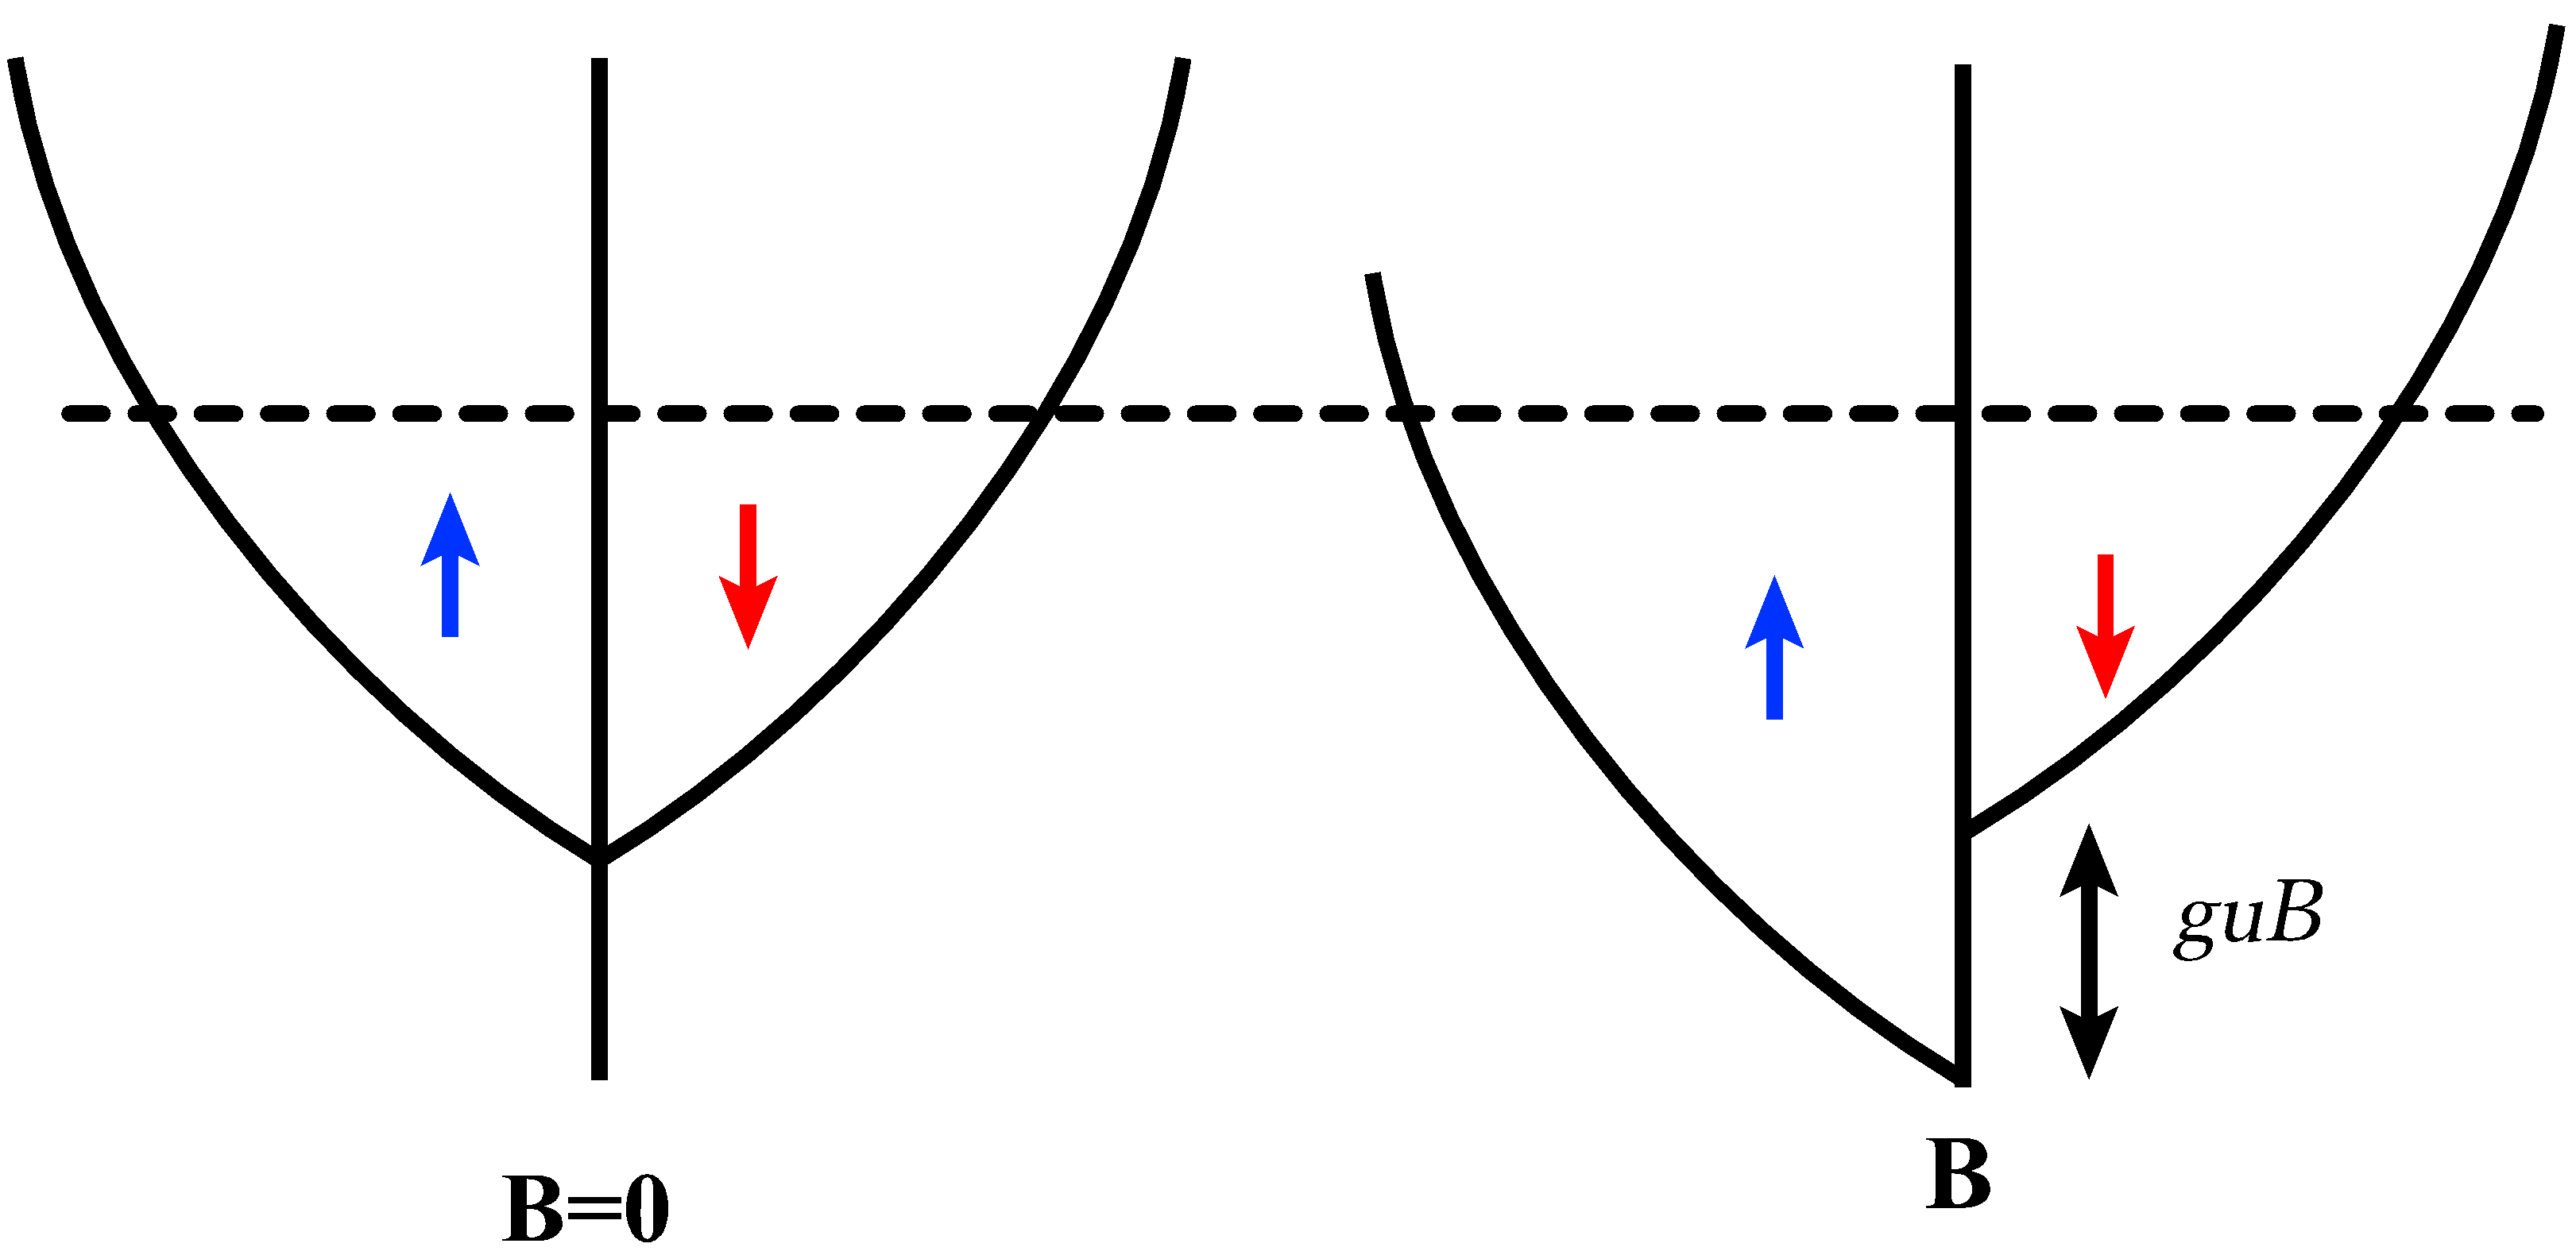
\includegraphics[scale=0.075]{PauliChi.png}
\caption{Change in the occupation of up/down spin states due to the applied field B.}
\end{figure}

The electrons can lower their energies by aligning parallel to the magnetic field. There is an imbalance in the number of up and down spins $n_{\uparrow/\downarrow}=n\pm\delta n$. The change in number of spin can be related to the change in energy by means of the density of states.
The density of states is defined as the number of states in the energy interval [$E,E+dE$]
\begin{equation}
D(E)=\dfrac{d n}{d E}
\end{equation}
Since the occupation change happens close to the Fermi level, we can relate the variation in number density $\delta n$ and the change in energy $dE$ through the density of states at the Fermi level.
\begin{equation}
\delta n =D_{F} dE = D_F g \mu_B B
\end{equation}
Thus the change in magnetization is 
\begin{equation}
\delta m = \dfrac{g \mu_B}{2} 2\delta n = D_F (g \mu_B)^2 B
\end{equation}
Therefore the Pauli paramagnetic susceptibility is
\begin{equation}
\chi_\mathrm{Pauli} = \dfrac{\delta m}{B} = D_F (g \mu_B)^2
\end{equation}

\end{document}